\subsection{Opportunistic Charging}
\label{subsec-opportunistic}

\begin{figure}[t]
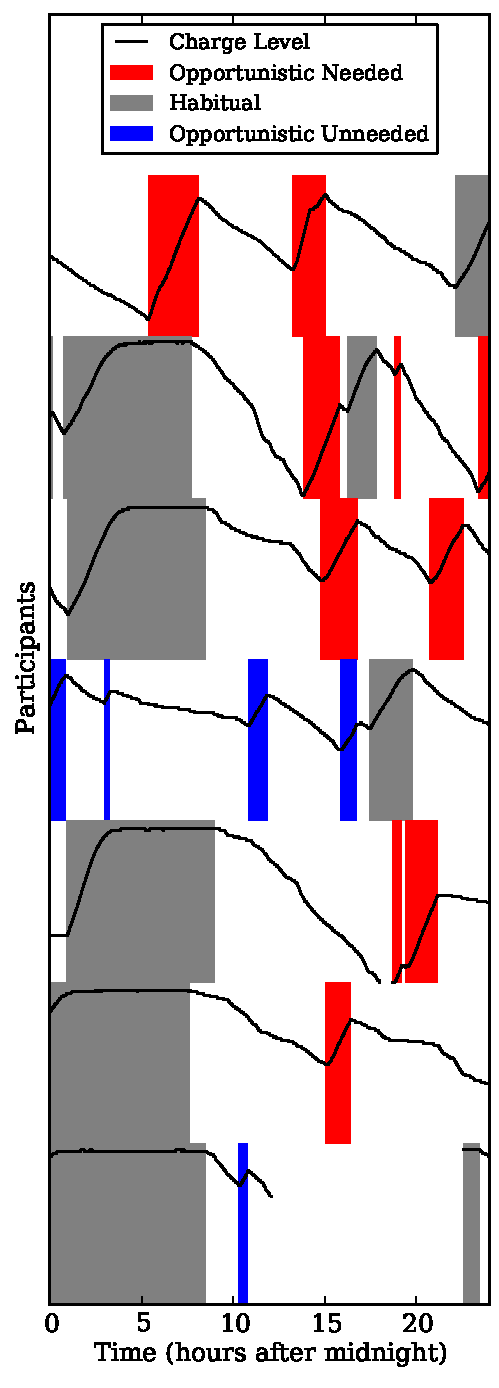
\includegraphics[width=\columnwidth]{./figures/power/opportunistic_charging/count_and_by_time/graph.pdf}
\caption{\textbf{Patterns of opportunistic charging.} Many users perform
opportunistic charging multiple times during the day.}
\label{fig-opportunistic-patterns}
\end{figure}

One way that users work around the battery limitations of their smartphone
devices is by finding new times and places to charge their phones: plugging
in at their desk at work, in the car during their commute, or at home before
a long night out. We refer to these charging sessions as
\textit{opportunistic} to distinguish them from \textit{habitual} nightly
charging. Assuming that many smartphone users encounter plug points
throughout the day, engaging in opportunistic charging becomes an additional
sign of energy awareness, and understanding opportunistic charging becomes
necessary to improving energy management on mobile devices.

\subsubsection{Seizing energy opportunities}

% 10 Dec 2012 : GWA : TODO : Numbers.

Figure~\ref{fig-opportunistic-patterns} shows that many users engage in
opportunistic charging. We define a charging session as opportunistic if is
long enough to not be spurious (over 10~minutes) but does not bring the
battery to a fully-charged state, indicating that the user disconnected the
device before charging could finish. Of the 79 charging sessions we observed,
35 (44\%) were opportunistic by this definition. 11 of 16 participants
engaged in opportunistic charging at some point during our experiment.

% 10 Dec 2012 : GWA : TODO : Numbers.

Opportunistic charging may be a response to an anticipated need for more
smartphone battery power: the student who plugs her smartphone in for a brief
charge before a night out. Our data also allowed us to examine how many of
these opportunistic charging sessions were necessary to bridge the gap to the
next full charge. We found that 15 of the 35 (42\%) of the opportunistic
charges we observed were necessary. We believe that this indicates that
participants have responded to their smartphones' battery limitations by
engaging in conservative charging behavior, grabbing power whenever possible.

\begin{figure*}[t]
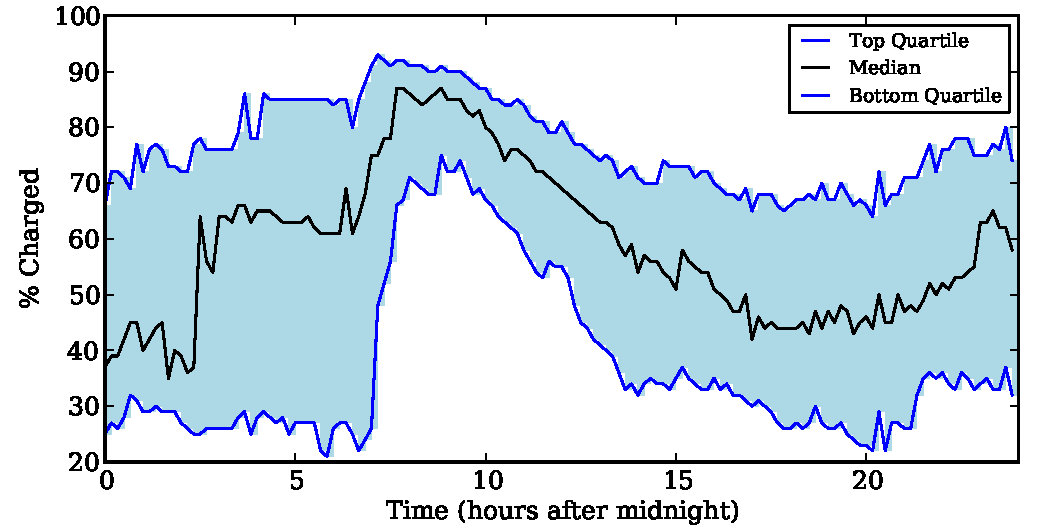
\includegraphics[width=\textwidth]{./figures/power/opportunistic_charging/max_difference/graph.pdf}
\caption{\textbf{Charge difference between participants during one day.} The
graph plots the top and bottom quartiles as well as the median. A significant
spread is present on the testbed throughout the day.}
\label{fig-opportunisticspread}
\end{figure*}

Combining opportunistic charging combined with the varied rhythms of our
participants creates a second interesting effect: at any given point on
\PhoneLab{} there is a wide disparity in the amount of power available on
different phones. Figure~\ref{fig-opportunisticspread} displays the top,
bottom, and middle (median) quartiles for a single day on \PhoneLab{}. Only
phones that are discharging are shown, which explains the sharp increase
between 6~and~10AM as participants end nightly charging cycles.  As the graph
indicates, there is a high chance that two smartphones that encounter each
other have very different battery levels.

\subsubsection{Future experiments}

We are not the first to note opportunistic charging
patterns~\cite{banerjee:ubicomp:2007, rahmati:mobilehci:2007}, but we believe
\PhoneLab{} can be used to address several interesting questions raised by
opportunistic charging. First, why do users engage in this practice? By
monitoring charging patterns an experiment could prompt users to indicate why
they were charging their phone after opportunistic charging sessions. This
would help shed more light as to the motivations of smartphone users and
their evolving relationship with power.

Second, new protocols might seek to use the increased charging differentials
as a result of opportunistic charging to establish a distributed energy
market. Phones with spare power and users that engage in opportunistic charge
frequently may agree to help another phone with less power conserve its
battery level---by switching WiFi access points, providing GPS coordinates or
acting as a real for cellular data---in exchange for assistance when the
tables are turned. Platform experiments on \PhoneLab{} could evaluate the
effectiveness of collaborative mobile energy management on a large and dense
testbed.
